% Chapter 3 - Design and Implementation (Defense Presentation)
% Use this for presentation slides

\section{Chapter 3}
\begin{frame}
\centering
\Huge \textbf{Design and Implementation}
\end{frame}

% ============================================
% Section: System Architecture
% ============================================
\subsection{System Architecture}

\begin{frame}{System Architecture Overview}
\begin{itemize}
    \item \textbf{Three-Tier Architecture}
    \begin{itemize}
        \item Presentation Layer: React Frontend
        \item Application Layer: Express.js Backend
        \item Data Layer: MongoDB Database
    \end{itemize}
    \vspace{0.5cm}
    \item \textbf{Communication}
    \begin{itemize}
        \item RESTful API architecture
        \item JSON data exchange format
    \end{itemize}
    \vspace{0.5cm}
    \item \textbf{Security}
    \begin{itemize}
        \item Google OAuth 2.0 authentication
        \item JWT token-based session management
    \end{itemize}
\end{itemize}
\end{frame}

\begin{frame}{Architecture Diagram}
\begin{center}
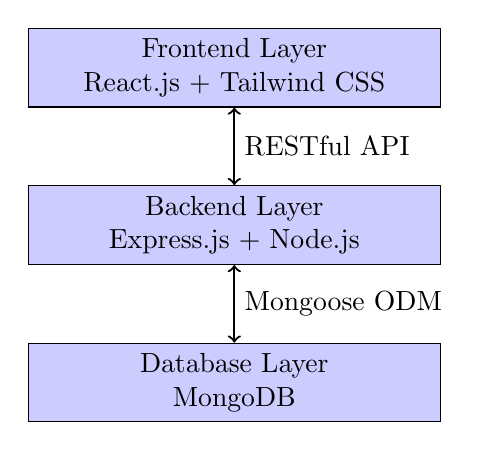
\begin{tikzpicture}[node distance=2cm, auto,
    layer/.style={rectangle, draw, fill=blue!20, text width=5cm, text centered, minimum height=1cm}]
    
    \node[layer] (frontend) {Frontend Layer\\React.js + Tailwind CSS};
    \node[layer, below of=frontend] (backend) {Backend Layer\\Express.js + Node.js};
    \node[layer, below of=backend] (database) {Database Layer\\MongoDB};
    
    \draw[<->, thick] (frontend) -- node[right] {RESTful API} (backend);
    \draw[<->, thick] (backend) -- node[right] {Mongoose ODM} (database);
\end{tikzpicture}
\end{center}
\end{frame}

% ============================================
% Section: System Requirements
% ============================================
\subsection{System Requirements}

\begin{frame}{Functional Requirements}
\begin{itemize}
    \item \textbf{User Authentication}
    \begin{itemize}
        \item Google OAuth login integration
        \item JWT-based session management
        \item User profile management
    \end{itemize}
    
    \item \textbf{Vehicle Management}
    \begin{itemize}
        \item Vehicle listing with photo uploads
        \item Multi-step vehicle registration form
        \item Vehicle search and filtering
    \end{itemize}
    
    \item \textbf{Booking System}
    \begin{itemize}
        \item Booking lifecycle management
        \item Real-time availability checking
        \item Booking conflict resolution
    \end{itemize}
    
    \item \textbf{Payment Processing}
    \begin{itemize}
        \item Demo payment system
        \item Transaction history tracking
    \end{itemize}
\end{itemize}
\end{frame}

\begin{frame}{Non-Functional Requirements}
\begin{itemize}
    \item \textbf{Security}
    \begin{itemize}
        \item HTTPS in production environment
        \item Password hashing with bcrypt
        \item Input validation and sanitization
        \item JWT token expiration (7 days)
    \end{itemize}
    
    \item \textbf{Maintainability}
    \begin{itemize}
        \item MVC (Model-View-Controller) architecture
        \item Modular code structure
        \item Comprehensive documentation
    \end{itemize}
    
    \item \textbf{Performance}
    \begin{itemize}
        \item Database indexing for faster queries
        \item API response pagination
        \item Optimized asset loading
    \end{itemize}
\end{itemize}
\end{frame}

% ============================================
% Section: Technology Stack
% ============================================
\subsection{Technology Stack}

\begin{frame}{Technology Stack}
\begin{columns}
\column{0.5\textwidth}
\textbf{Frontend Technologies}
\begin{itemize}
    \item React.js (UI Framework)
    \item Tailwind CSS (Styling)
    \item Axios (HTTP Client)
    \item React Router (Navigation)
    \item Context API (State Management)
\end{itemize}

\column{0.5\textwidth}
\textbf{Backend Technologies}
\begin{itemize}
    \item Node.js (Runtime)
    \item Express.js (Framework)
    \item MongoDB (Database)
    \item Mongoose (ODM)
    \item Multer (File Upload)
    \item JWT (Authentication)
\end{itemize}
\end{columns}
\end{frame}

% ============================================
% Section: Database Design
% ============================================
\subsection{Database Design}

\begin{frame}{Database Schema}
\textbf{Primary Collections:}
\begin{enumerate}
    \item \textbf{Users Collection}
    \begin{itemize}
        \item User credentials and profile
        \item Google OAuth information
        \item Verification status
    \end{itemize}
    
    \item \textbf{Vehicles Collection}
    \begin{itemize}
        \item Vehicle details and specifications
        \item Owner reference (ObjectId)
        \item Photo URLs and pricing
    \end{itemize}
    
    \item \textbf{Bookings Collection}
    \begin{itemize}
        \item Booking dates and status
        \item User and Vehicle references
        \item Payment information
    \end{itemize}
    
    \item \textbf{Payments Collection}
    \begin{itemize}
        \item Transaction details
        \item Fare breakdown
        \item Payment status
    \end{itemize}
\end{enumerate}
\end{frame}

\begin{frame}{Entity Relationship}
\begin{center}
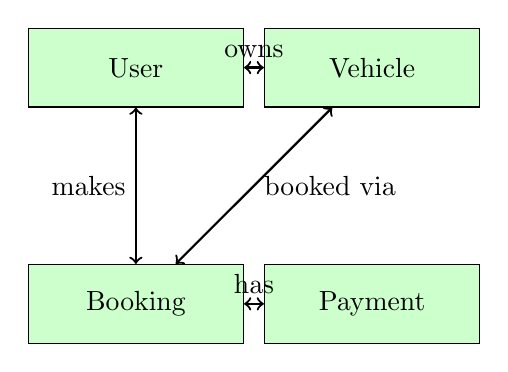
\begin{tikzpicture}[node distance=3cm, auto,
    entity/.style={rectangle, draw, fill=green!20, text width=2.5cm, text centered, minimum height=1cm}]
    
    \node[entity] (user) {User};
    \node[entity, right of=user] (vehicle) {Vehicle};
    \node[entity, below of=user] (booking) {Booking};
    \node[entity, right of=booking] (payment) {Payment};
    
    \draw[<->, thick] (user) -- node[above] {owns} (vehicle);
    \draw[<->, thick] (user) -- node[left] {makes} (booking);
    \draw[<->, thick] (vehicle) -- node[right] {booked via} (booking);
    \draw[<->, thick] (booking) -- node[above] {has} (payment);
\end{tikzpicture}
\end{center}
\end{frame}

% ============================================
% Section: Implementation Details
% ============================================
\subsection{Implementation Details}

\begin{frame}{Authentication Implementation}
\textbf{Google OAuth 2.0 Flow:}
\begin{enumerate}
    \item User initiates login via Google
    \item Redirect to Google authentication page
    \item User grants permissions
    \item Backend receives authorization code
    \item Exchange code for user information
    \item Generate JWT token (7-day expiry)
    \item Return token to frontend
    \item Store token in localStorage
\end{enumerate}

\vspace{0.3cm}
\textbf{JWT Token Management:}
\begin{itemize}
    \item Middleware validates token on protected routes
    \item Automatic token refresh mechanism
    \item Secure token storage in browser
\end{itemize}
\end{frame}

\begin{frame}{Vehicle Management System}
\textbf{Multi-Step Vehicle Registration:}
\begin{enumerate}
    \item Basic vehicle information
    \item Vehicle specifications and features
    \item Pricing and availability
    \item Photo upload (using Multer)
    \item Review and submit
\end{enumerate}

\vspace{0.3cm}
\textbf{File Upload Handling:}
\begin{itemize}
    \item Multer middleware for secure uploads
    \item Image validation (type, size)
    \item Storage in public directory
    \item Database URL reference storage
\end{itemize}
\end{frame}

\begin{frame}{Booking Management System}
\textbf{Booking Lifecycle State Machine:}
\begin{itemize}
    \item \texttt{PENDING} - Initial booking request
    \item \texttt{CONFIRMED} - Accepted by vehicle owner
    \item \texttt{CANCELLED} - Cancelled by either party
    \item \texttt{COMPLETED} - Rental period finished
\end{itemize}

\vspace{0.3cm}
\textbf{Conflict Checking Algorithm:}
\begin{enumerate}
    \item Query existing bookings for vehicle
    \item Check date range overlaps
    \item Validate booking constraints
    \item Return availability status
    \item Prevent double booking
\end{enumerate}
\end{frame}

\begin{frame}{Payment System}
\textbf{Demo Payment Flow:}
\begin{enumerate}
    \item Calculate fare based on duration
    \item Display payment breakdown
    \item Simulate payment processing
    \item Create transaction record
    \item Update booking status
    \item Send confirmation
\end{enumerate}

\vspace{0.3cm}
\textbf{Fare Calculation:}
\begin{itemize}
    \item Base fare = Vehicle daily rate × Number of days
    \item Service fee = 10\% of base fare
    \item Total = Base fare + Service fee
    \item Transaction stored in Payments collection
\end{itemize}
\end{frame}

% ============================================
% Section: API Design
% ============================================
\subsection{API Design}

\begin{frame}{RESTful API Endpoints}
\begin{table}
\scriptsize
\begin{tabular}{|l|l|l|}
\hline
\textbf{Endpoint} & \textbf{Method} & \textbf{Purpose} \\
\hline
/api/auth/google & POST & Google OAuth login \\
/api/auth/register & POST & User registration \\
/api/vehicles & GET & List all vehicles \\
/api/vehicles/:id & GET & Get vehicle details \\
/api/vehicles & POST & Create vehicle listing \\
/api/bookings & GET & User's bookings \\
/api/bookings & POST & Create new booking \\
/api/bookings/:id & PUT & Update booking status \\
/api/payments & POST & Process payment \\
/api/recommendations & GET & Get vehicle recommendations \\
\hline
\end{tabular}
\end{table}
\end{frame}

% ============================================
% Section: Security Implementation
% ============================================
\subsection{Security Implementation}

\begin{frame}{Security Measures}
\begin{itemize}
    \item \textbf{Authentication Security}
    \begin{itemize}
        \item OAuth 2.0 for third-party authentication
        \item JWT with secure signature
        \item Token expiration and refresh
    \end{itemize}
    
    \item \textbf{Data Security}
    \begin{itemize}
        \item Password hashing with bcrypt
        \item Input validation using express-validator
        \item SQL injection prevention via Mongoose
        \item XSS protection with sanitization
    \end{itemize}
    
    \item \textbf{API Security}
    \begin{itemize}
        \item Authentication middleware on protected routes
        \item CORS configuration
        \item Rate limiting (future enhancement)
    \end{itemize}
\end{itemize}
\end{frame}

% ============================================
% Section: Development Methodology
% ============================================
\subsection{Development Methodology}

\begin{frame}{Development Approach}
\textbf{Agile Development Process:}
\begin{itemize}
    \item Iterative development cycles
    \item Feature-based implementation
    \item Continuous testing and refinement
\end{itemize}

\vspace{0.3cm}
\textbf{Version Control:}
\begin{itemize}
    \item Git for version control
    \item Feature branching strategy
    \item Regular commits and documentation
\end{itemize}

\vspace{0.3cm}
\textbf{Testing Strategy:}
\begin{itemize}
    \item Manual testing of all features
    \item API testing using Postman
    \item Browser compatibility testing
\end{itemize}
\end{frame}

% ============================================
% Conclusion Slide for Chapter 3
% ============================================
\begin{frame}{Chapter 3 Summary}
\begin{itemize}
    \item Implemented three-tier client-server architecture
    \item Designed scalable database schema with MongoDB
    \item Integrated Google OAuth for secure authentication
    \item Developed comprehensive booking system with conflict checking
    \item Created RESTful API with proper security measures
    \item Followed MVC pattern for maintainable code
\end{itemize}

\vspace{0.5cm}
\centering
\textbf{Key Achievement:} Fully functional vehicle sharing platform with secure authentication, booking management, and payment processing.
\end{frame}
